\setlength{\footskip}{8mm}

\chapter{Introduction}

\section{Overview}

Data analysis is an very robust topic in the field of data science and encompasses the various mathematical functions. The functions are statistical in nature and are performed on the data obtained. The goal of data analytics is to support (or reject) the hypothesis which the data scientist postulates.
“ By processing a steady stream of real-time data, organizations can make time-sensitive decisions faster than ever before, monitor emerging trends, course-correct rapidly and jump on new business opportunities.” [BIG Data Analytics: A Framework for Unstructured Data Analysis pdf]

This paper tries to enlist most of the up-to-date techniques used by researchers and mathematicians to make sense of the data. Also the paper presents them in three groups of analytics.
But then there arises a question which is, why the need for data analytics ? Well, to answer that the paper proposes the literature from an article of Kdnuggets \shortcite{KDnuggets}.

Data analytics is already the next big disrupter in the financial sector~\shortcite{Forbes2017}. New startups are build solutions to automate mundane manual tasks of reconciliations and consolidations. Artificial intelligence is helping companies to redesign the traditional process flows and restructure work-flows for optimization. With complex algorithms of machine learning, artificial intelligence, ``Bot's`` are designed which learn the product usage and popularity among customers. These ``Bot's`` can also interact autonomously to users and deduce patterns of interaction.
Such an exisiting example is cited in Cnbc's article~\shortcite{BOA2016}, about Bank of America deploying ``Erica`` an digital assistant based on models of artificial intelligence.

According to Paul following are use cases  of data analytics :
\begin{enumerate}
	\item Analytics powers our decisions – we do not need to guess while making bold new decisions, we should use the information from data at hand.
	\item Your data analysis weighs down your opponent's argument.
	\item Cut down on loss making ventures with data analytics.
	\item Can be applied to all domains be it health-care, banking, marketing, sales, operations etc.
\end{enumerate}

On the scenario when describing Data analytics it is very important to put the focus on Hypothesis.

Shown in the table~\ref{tableDMusecase} is some business areas 


\begin{table}[H]
	\centering
%	\hskip-1.8cm
	\begin{tabular}{|p{4cm}|p{4cm}|l|}
		\hline
		\textbf{Application area} & \textbf{Applications} & \textbf{Specifics}\\
		\hline
		Insurance & Fraud detection & Identify claims meriting investigation\\
		\hline
		Telecom & Churn & Identify likely customer turnover\\
		\hline
		Telemarketing & On-line information & Aid telemarketers with easy data access\\
		\hline
		Human resource management & Churn & Identify potential employee turnover\\
		\hline
		\multirow{2}{4em}{Retail}  & Affinity positioning & Position product effectively\\
		& Cross-selling & Find more products for customers\\
		\hline
		\multirow{2}{4em}{Banking} & Customer relationship management & Identify customer value\\
		&& Develop programs to maximize revenue\\
		\hline
		Credit card management & Lift & Identify effective market segments\\
		& Churn & Identify likely customer turnover\\
		\hline
	\end{tabular}
	\caption{Data mining use cases}
	\label{tableDMusecase}
\end{table}
	
Figure \ref{fig:data-analytics} is a view of the data analytics with respect to the main fields.

\begin{figure}[H]
	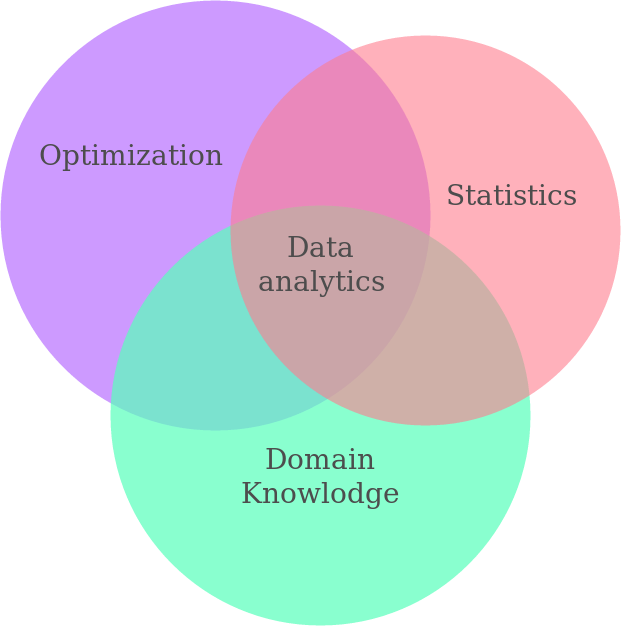
\includegraphics[scale = 0.6]{figures/AnalyticsDomain.png}
	\centering
	\caption{Data Analytics}
	\label{fig:data-analytics}
\end{figure}
\FloatBarrier

Below we see a representations for the advanced analytics and business analytics~\ref{fig:rapidminer-aa}.

\begin{figure}[H]
	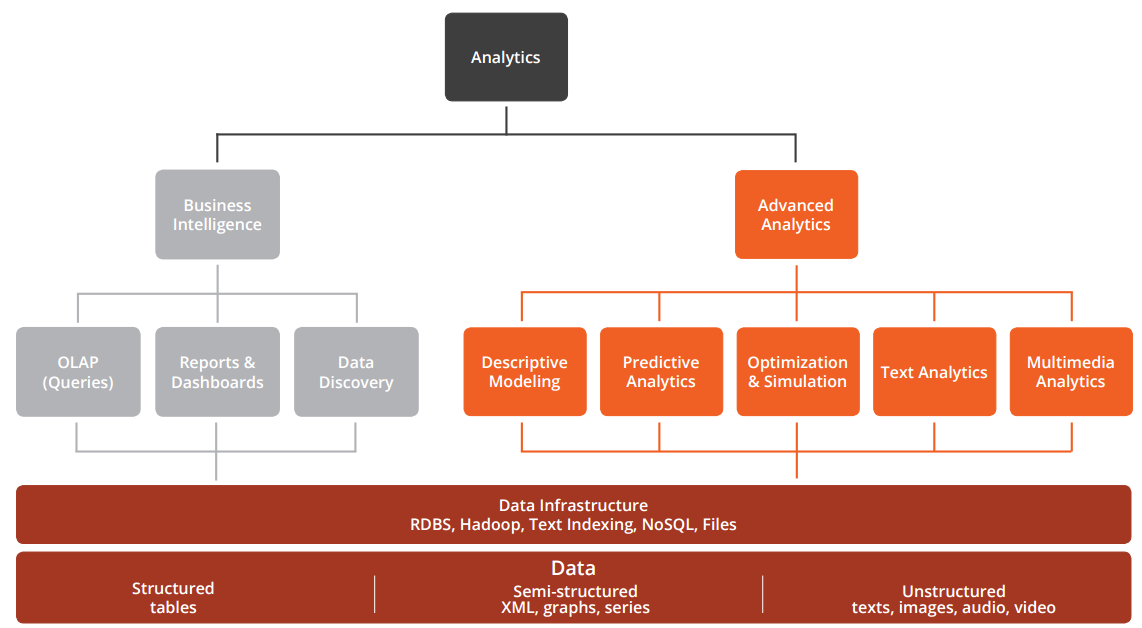
\includegraphics[scale=0.4]{figures/RapidMiner_AdvancedAnalytics_new.png}
	\caption{Advanced analytics}
	\label{fig:rapidminer-aa}
\end{figure}


\section{Objectives}

The overall objective of the study report is to build an understanding of the tools and techniques of analytics used by financial analysts and institutions. This study presents a brief of the current state of affairs analytics and subsequently a study of the techniques. Also there is a demonstration of some common methods.

